\documentclass[letterpaper,12pt,oneside]{article}\usepackage[]{graphicx}\usepackage[]{color}
%% maxwidth is the original width if it is less than linewidth
%% otherwise use linewidth (to make sure the graphics do not exceed the margin)
\makeatletter
\def\maxwidth{ %
  \ifdim\Gin@nat@width>\linewidth
    \linewidth
  \else
    \Gin@nat@width
  \fi
}
\makeatother

\definecolor{fgcolor}{rgb}{0.345, 0.345, 0.345}
\newcommand{\hlnum}[1]{\textcolor[rgb]{0.686,0.059,0.569}{#1}}%
\newcommand{\hlstr}[1]{\textcolor[rgb]{0.192,0.494,0.8}{#1}}%
\newcommand{\hlcom}[1]{\textcolor[rgb]{0.678,0.584,0.686}{\textit{#1}}}%
\newcommand{\hlopt}[1]{\textcolor[rgb]{0,0,0}{#1}}%
\newcommand{\hlstd}[1]{\textcolor[rgb]{0.345,0.345,0.345}{#1}}%
\newcommand{\hlkwa}[1]{\textcolor[rgb]{0.161,0.373,0.58}{\textbf{#1}}}%
\newcommand{\hlkwb}[1]{\textcolor[rgb]{0.69,0.353,0.396}{#1}}%
\newcommand{\hlkwc}[1]{\textcolor[rgb]{0.333,0.667,0.333}{#1}}%
\newcommand{\hlkwd}[1]{\textcolor[rgb]{0.737,0.353,0.396}{\textbf{#1}}}%

\usepackage{framed}
\makeatletter
\newenvironment{kframe}{%
 \def\at@end@of@kframe{}%
 \ifinner\ifhmode%
  \def\at@end@of@kframe{\end{minipage}}%
  \begin{minipage}{\columnwidth}%
 \fi\fi%
 \def\FrameCommand##1{\hskip\@totalleftmargin \hskip-\fboxsep
 \colorbox{shadecolor}{##1}\hskip-\fboxsep
     % There is no \\@totalrightmargin, so:
     \hskip-\linewidth \hskip-\@totalleftmargin \hskip\columnwidth}%
 \MakeFramed {\advance\hsize-\width
   \@totalleftmargin\z@ \linewidth\hsize
   \@setminipage}}%
 {\par\unskip\endMakeFramed%
 \at@end@of@kframe}
\makeatother

\definecolor{shadecolor}{rgb}{.97, .97, .97}
\definecolor{messagecolor}{rgb}{0, 0, 0}
\definecolor{warningcolor}{rgb}{1, 0, 1}
\definecolor{errorcolor}{rgb}{1, 0, 0}
\newenvironment{knitrout}{}{} % an empty environment to be redefined in TeX

\usepackage{alltt}
\usepackage[paperwidth=8.5in,paperheight=11in,top=1in,bottom=1in,left=1in,right=1in]{geometry}
\usepackage{setspace}
\usepackage[colorlinks=true,allcolors=Blue]{hyperref}
\usepackage[usenames,dvipsnames]{xcolor}
\usepackage{indentfirst}
\usepackage{titlesec}
\usepackage{multirow}
\usepackage{booktabs}
\usepackage{graphicx}
\usepackage{verbatim}
\usepackage{rotating}
\usepackage{tabularx}
\usepackage{outlines}
\usepackage{lineno}
\usepackage{array}
\usepackage{times}
\usepackage{cleveref}
\usepackage{acronym}
\usepackage[position=t]{subfig}
\usepackage{paralist}
\usepackage[noae]{Sweave}
\usepackage{natbib}
\usepackage{array}
\usepackage{pdflscape}
\usepackage{bm}
\usepackage{showlabels}
\bibpunct{(}{)}{,}{a}{}{,}

% page margins and section title formatting
\linespread{2}
\setlength{\footskip}{0.5in}
\titleformat*{\section}{\Large\bf\em}
\titleformat*{\subsection}{\singlespace\large\bf}
\titleformat*{\subsubsection}{\singlespace\normalsize\bf\em}
\titlespacing{\section}{0in}{0in}{0in}
\titlespacing{\subsection}{0in}{0in}{0in}
\titlespacing{\subsubsection}{0in}{0in}{0in}

% cleveref options
\crefname{table}{Table}{Tables}
\crefname{figure}{Fig.}{Figs.}
\renewcommand{\figurename}{Fig.}

% aliased citations
\defcitealias{HagyIR}{Hagy, In review}
\defcitealias{USEPA98}{USEPA, 1998}

%acronyms
\acrodef{DEM}{Digital Elevation Model}
\acrodef{EPA}{Environmental Protection Agency}
\acrodef{doc}[DoC]{depth of colonization}
\acrodef{GIS}{Geographic Information System}
\acrodef{IWR}{Impaired Waters Rule}
\acrodef{MSL}{mean sea level}
\acrodef{NAVD88}{North American Vertical Datum of 1988}
\acrodef{NOAA}{National Oceanic and Atmospheric Administration}

%knitr options


\IfFileExists{upquote.sty}{\usepackage{upquote}}{}
\begin{document}

\raggedbottom
\linenumbers
\raggedright
\urlstyle{same}
\setlength{\parindent}{0.5in}
\renewcommand\refname{References \vspace{12pt}}

\begin{singlespace}
\title{{\bf {\Large Improved estimates of seagrass light requirements using reproducible and spatially-referenced depths of colonization}}}
\author{
  {\bf {\normalsize Marcus W. Beck$^1$, James D. Hagy III$^2$}}
  \\\\{\textit {\normalsize $^1$ORISE Research Participation Program}}
  \\{\textit {\normalsize USEPA National Health and Environmental Effects Research Laboratory}}
  \\{\textit {\normalsize Gulf Ecology Division, 1 Sabine Island Drive, Gulf Breeze, FL 32561}}
	\\{\textit {\normalsize Phone: 850-934-2480, Fax: 850-934-2401, Email: \href{mailto:beck.marcus@epa.gov}{beck.marcus@epa.gov}}}
  \\\\{\textit {\normalsize $^2$USEPA National Health and Environmental Effects Research Laboratory}}
	\\{\textit {\normalsize Gulf Ecology Division, 1 Sabine Island Drive, Gulf Breeze, FL 32561}}
	\\{\textit {\normalsize Phone: 850-934-2455, Fax: 850-934-2401, Email: \href{mailto:hagy.jim@epa.gov}{hagy.jim@epa.gov}}}
	}
\date{}
\maketitle
\end{singlespace}
\clearpage

\section{Introduction}

Issues related to excessive nutrient pollution have motivated a substantial amount of research to understand and address impacts on coastal waters.  Eutrophication, defined as an increase in the rate of supply of organic matter to an ecosystem \citep{Nixon95}, is primarily caused by anthropegenic inputs of limiting nutrients that exceed background concentrations of receiving waters.  Adverse impacts on aquatic resources are well-documented and have included increased occurrence in the frequency and severity of harmfal algal blooms \citep{Cloern96}, reduction of dissolved oxygen necessary to support heterotrophic organisms \citep{Justic87,Diaz08}, and loss of ecosystem functioning through food web simplification \citep{Tewfik07}. Although management activities have been successful in mitigating or reversing eutrophication impacts (e.g., \citealt{Greening06}), the evaluation of response endpoints remains an important topic given that ecosystem changes in relation to different nutrient regimes are not fully understood nor anticipated \citep{Duarte09}.  The most appropriate indicators of ecosystem response may be those that exhibit clear biological linkages with water quality changes, such that the potential effects of management actions can be unambiguously characterized through known cause and effect pathways.  Critical management decisions may be forced by tentative assessments, political or societal pressures, or qualitative criteria in the absence of empirical methods to identify adequate indicators of ecosytem response \citep{Duarte09}.  

The ecosystem services provided by seagrasses as well as their sensitivity to water quality changes has contributed to their proliferation as biological response endpoints for eutrophication.  Seagrasses are ecosystem engineers \citep{Jones94,Koch01} that serve a structural and functional role in altering aquatic habitat often through multiple feedback mechanisms with other ecosystem components.  For example, seagrass beds create habitat for juvenile fish and crabs by reducing wave action and stabilizing sediment \citep{williams01,Hughes09}.  Seagrasses also respond to changes in water clarity through direct physiological linkages with light availability.  In short, increased nutrient loading contributes to reductions in water clarity through increased algal concentrations, inhibiting the growth of seagrass through light limitation \citep{Duarte95}.  Empirical relationships between nutrient loading, water clarity, light requirements, and the maximum depth of seagrass colonization have been identified \citep{Duarte91,Kenworthy96,Choice14}, such that quantitative standards can be developed to maintain light regimes sufficient for seagrass growth targets \citep{Steward05}.  Conversely, seagrass depth limits have formed the basis of quantititative criteria for nutrient load targets \citep{Janicki96}.  Contrasted with numeric standards for nutrients and phytoplankon, seagrass-based criteria may be more practical for developing water quality standards given that seagrasses are integrative of system-wide conditions over time and less variable with changes in nutrient regimes \citep{Duarte95}.  

The development of numeric criteria and standards for coastal waters has been a management priority within the United States \citepalias{USEPA98} and internationally \citep{WFD00}.  Numerous agencies and management programs have developed a variety of techniques for estimating seagrass depth limits as a basis for establishing numeric criteria, either as restoration targets or for identifying critical load limits.  Such efforts have been useful for site-specific approaches where the analysis needs are driven by a particular management or research context \citep[e.g.,][]{Iverson86,Hale04}. However, a lack of standardization among methods has prevented broad-scale comparisons between regions and has even contributed to discrepancies between measures of depth limits based on the chosen technique.  For example, seagrass depth limits based on in situ techniques can vary with the sampling device \citep{Spears09}.  Despite the availability of data, techniques for estimating seagrass depth of colonization using remotely sensed data have not been extensively developed.  Such techniques have the potential to facilitate broad-scale comparisons between regions given the spatial coverage and annual availability of many products.  For example, recent analyses by \citetalias{HagyIR} have shown that standardized techniques using seagrass coverage maps and bathymetric data can be developed to compare growth patterns over time among different coastal regions of Florida.  Such methods show promise, although further development to improve the spatial resolution of the analysis are needed.  Specifically, methods for estimating seagrass depth limits should be reproducible for broad-scale comparisons, while also maintaining flexibility for site-specific estimates depending on management needs.

Reproducible and empirical approaches can be developed to provide more consistent estimates of seagrass depth limits for restoration targets or criteria development. We describe a method for estimating seagrass depth of colonization using information-rich datasets to create a spatially explicit and repeatable estimate.  In particular, methods described in \citetalias{HagyIR} are improved upon by creating a flexible and repeatable technique for estimating seagrass depth limits from coverage maps and bathymetric data. The specific objectives are to\begin{inparaenum}[1\upshape)]
\item describe the method for estimating seagrass depth limits within a relevant spatial context, 
\item apply the technique to four distinct regions of Florida to illustrate improved clarity of description for seagrass growth patterns, and
\item develop a spatially coherent relationship between depth limits and water clarity for the case studies.  
\end{inparaenum}
Overall, these methods are expected to inform the development of water quality criteria based on empirical relationships of seagrass depth limits with water clarity over time.  The method is applied to data from Florida although the technique is transferable to other regions with comparable data. 

\section{Methods}

Development of a spatially-referenced approach to estimate seagrass \ac{doc} relied extensively on data and partially on methods described in \citetalias{HagyIR}.  The following is a summary of locations and data sources, methods and rationale for incorporating spatial information in seagrass \ac{doc} estimates, and evaluation of the approach including relationships with water clarity.   

\subsection{Locations and data sources}

Four unique locations were chosen for the analysis: Choctowatchee Bay (Panhandle), Big Bend region (northeast Gulf of Mexico), Tampa Bay (central Gulf Coast of Florida), and Indian River Lagoon (east coast) (\cref{tab:seg_summ,fig:seg_all}).  These locations represent different geographic regions in the state, in addition to having available data and observed gradients in water clarity that contribute to hetereogeneity in seagrass growth patterns.  For example, the Big Bend region was chosen based on location near an outflow of the Steinhatchee River where higher concentrations of dissolved organic matter are observed.  Seagrasses near the outflow were observed to grow at shallower depths as compared to locations far from the river source.  Coastal regions and estuaries in Florida are partitioned as distinct spatial units based on a segmentation scheme developed by US \ac{EPA} for the development of numeric nutrient criteria.  One segment from each geographic location was used to describe the approach for estimating seagrass \ac{doc} and to evaluate variation in growth patterns \ac{doc}.  The segments included 0303 (Choctowatchee Bay), 0820 (Big Bend region), 0902 (Tampa Bay), and 1502 (Indian River Lagoon), where the first two digits indicate the estuary and the last two digits indicate the segment within the estuary.  Each segment was a smaller unit within a larger estuary or coastal region.   

Data used to estimate seagrass \ac{doc} were primarily obtained from publically available \ac{GIS} products.  At the most generic level, spatially-referenced information describing seagrass aerial coverage combined with co-located bathymetric depth information were used to estimate \ac{doc}.  These data products are available in coastal regions of Florida through the US Geological Survey, Florida Department of Environmental Protection, and watershed management districts.  Data are generally more available in larger estuaries that are of specific management concern.  For example, seagrass coverage data are available from 1950 (Tampa Bay) to present day (multiple estuaries), with more recent products available at annual or  biennial intervals.  Seagrass coverage maps are less frequent in areas with lower population densities (e.g., Big Bend region) or where seagrass is naturally absent (northeast Florida).  Seagrass maps were produced using photo-interpretations of aerial images to categorize coverage as absent, discontinuous (patchy), or continuous.  For this analysis, we considered seagrass coverage as being only present (continuous and patchy) or absent since the former did not represent unequivocal categories between regions. 

Seagrass coverage maps were combined with bathymetric depth layers to characterize location and depth of growth in each location.  Bathymetric depth layers for each location were obtained from the National Oceanic and Atmospheric Administration's (\acsu{NOAA}) National Geophysical Data Center as either \acp{DEM} or raw sounding data from hydroacoustic surveys.  Tampa Bay data provided by the Tampa Bay National Estuary Program are described in \citet{Tyler07}. Bathymetric data for the Indian River Lagoon were obtained from the St. John's Water Management District \citep{CPE97}.  \ac{NOAA} products were referenced to mean lower low water, whereas Tampa Bay data were referenced to the \ac{NAVD88} and the Indian River Lagoon data were referenced to mean sea level.  Depth layers were combined with seagrass coverage layers using standard union techniques for raster and vector layers in ArcMap 10.1 \citep{ESRI12}.  To reduce computation time, depth layers were first masked using a 1 km buffer of the seagrass coverage layer.  The final layer used for analysis was a point layer with attributes describing location (latitude, longitude, segment), depth (m), and seagrass (present, absent).  All spatial data were referenced to the North American Datum of 1983 as geographic coordinates.  Depth values in each seagrass layer were further adjusted from the relevant vertical reference datum to local \ac{MSL} using the \ac{NOAA} VDatum tool (\url{http://vdatum.noaa.gov/}).

\subsection{Segment-based estimates of seagrass depth of colonization}

\citetalias{HagyIR} describe an approach to estimate seagrass \ac{doc} for individual coastal segments.  The approach described herein is theoretically similar to the initial method, although the latter technique has a spatial resolution that uses segments as the smallest measurable unit.  Seagrass depth data described above are used to estimate maximum ($Z_{cMax}$) and median ($Z_{c50\%}$) seagrass \ac{doc}, where the maximum depth is defined as the deepest depth at which a ``significant'' coverage of seagrasses occured in a segment and the median depth is defined as the median depth occurring at the deep water edge. The seagrass depth points are grouped into bins and the proportion of points within each depth bin that contain seagrass are quantified.  Both seagrass \ac{doc} estimates are obtained from a plot of proportion of points occupied at each depth bin.  In general, the plot is characterized by a decreasing trend such that the proportion of occupied points by depth bin decreases and eventually flattens with increasing depth.  A regression is fit on this descending portion of the curve such that the intercept point on the x-axis is considered the maximum depth of colonization.  The median portion of this curve is considered the median depth of the deepwater edge of seagrass.   

Considerable spatial heterogeneity in the observed seagrass growth patterns suggests that a segment-wide estimate of seagrass \ac{doc} may be inadequate for fully characterizing growth patterns, particularly for the examples in the current analysis. \Cref{fig:wbid_doc} illustrates spatial variation in seagrass distribution  for a location in the Big Bend region of Florida.  Using methods in \citetalias{HagyIR}, the estimate for median seagrass \ac{doc} for the segment is over- and under-estimated for different locations.  In particular, \ac{doc} is greatly over-estimated at the outflow of the Steinhatchee River where high concentrations of dissolved organic matter reduce water clarity and naturally limit seagrass growth.  This example suggests that estimates of \ac{doc} may be needed at finer spatial scales to provide a more robust determination of restoration targets and nutrient criteria.  Although the current example is immediately relevant for the Big Bend region of Florida, the remaining examples discussed throughout also provide a justification for a more comprehensive assessment of seagrass growth patterns.  

\subsection{Estimating seagrass depth of colonization using spatial information}

The approach used to estimate seagrass \ac{doc} with spatial information has several key differences that make it distinct from the original method.  As before, seagrass \ac{doc} estimates are based on empirical measures of the frequency occurrence of seagrass with increasing depth.  The first difference is that maximum \ac{doc} is estimated using a logistic growth curve fit through the data, as compared to a simple linear regression in the previous example.  Second, a third measure describing the minimum depth of colonization was defined, in addition to median and maximum depth of growth.  The third and most important difference is that the estimates are assigned to discrete cartesian locations, using either a grid of points or as a single location of interest. Methods and implications of these differences are described below.                                   

The spatially-referenced approach for estimating \ac{doc} begins by creating a grid of points within the segment where the same process for estimating \ac{doc} is used for each point.  Alternatively, a single location of interest can be chosen rather than a grid-based design.  Seagrass depth data (i.e., merged bathymetric and seagrass coverage data) that are located within a set radius from the chosen locations are selected for estimating seagrass \ac{doc} values (\cref{fig:buff_ex}). The estimate for each location is quantified from a plot of the proportion of bathymetric soundings that contain seagrass at each depth bin (\cref{fig:est_ex1}).  Although the chosen radius for selecting depth points is problem-specific, the minimum radius must sample a sufficient number of points for estimating \ac{doc}.  In general, an appropriate radius will produce a plot that indicates a decrease in the proportion of points that are occupied by seagrass with increasing depth. An appropriate radius is also one that creates a sample area around each point that has minimal overlap with the seagrass depth data sampled by adjacent points.     

A curve is fit to the sampled depth points using non-linear regression to characterize the reduction in seagrass as a function of depth (\cref{fig:est_ex2}).  Specifically, a decreasing logistic growth curve is used with the assumption that seagrass decline with increasing depth is monotonic and asymptotic at the maximum depth of colonization. The curve is fit by minimizing the residual sums-of-squares with the Gauss-Newton algorithm \citep{Bates92} and user-supplied starting parameters that are an approximate estimate of the curve characteristics.  The model has the following form:
\begin{equation} \label{eqn:prop}
 Proportion = \frac{\alpha}{1 + \mathrm{e}^{{\left(\beta - Depth\right)/\gamma}}}
\end{equation}
where the proportion of points occupied by seagrass at each depth is defined by a logistic curve with an asymptote $\alpha$, a midpoint inflection $\beta$, and a scale parameter $\gamma$.  Starting values $\alpha$, $\beta$, and $\gamma$ were estimated empirically from the observed data.  

Finally, a simple linear curve is fit through the inflection point ($\beta$) of the logistic curve to estimate the three measures of depth of colonization (\cref{fig:est_ex3}).  The inflection point is considered the depth at which seagrass are decreasing at a maximum rate and is used as the slope of the linear curve.  Three measures describing seagrass growth characteristics are obtained. The maximum depth of seagrass colonization, $Z_{max}$, is the x-axis intercept of the linear curve.  The minimum depth of seagrass growth, $Z_{min}$, is the location where the linear curve intercepts the asymptote of the logistic growth curve.  This depth can be considered the start of the decline in seagrass coverage with increasing depth.  The median depth of seagrass colonization, $Z_{med}$, is the depth halfway between $Z_{min}$ and $Z_{max}$.  $Z_{med}$ was typically the inflection point of the logistic growth curve.  Functionally, each measure has specific ecological significance.  The median and maximum depth estimates describe the growth limitations of seagrasses as a function of water clarity, whereas minimum depth of growth was often where the highest percentage of seagrass coverage was observed in the sample.  Median and maximum depth estimates differ in that the former describes the median depth of the deep water edge, whereas the latter describes a nominal characterization of maximum depth independent of outliers.

Estimates for each of the three \ac{doc} measures are obtained only if specific criteria are met.  These criteria were implemented as a safety measure that ensures a sufficient amount and appropriate quality of data were used.  First, estimates were provided only if a sufficient number of seagrass depth points were present within the radius of the grid point to estimate a logistic growth curve.  This criteria applies to the sample size as well as the number of points with seagrass in the sample.  The curve could not be estimated for small samples or if an insufficient number of points contained seagrass regardless of sample size.  Second, estimates were provided only if an inflection point was present on the logistic curve within the range of the sampled depth data.  This criteria applied under two scenarios where the curve was estimated but a trend was not adequately described by the sampled data.  That is, a curve could be estimated that described only the initial decrease in points occupied as a function of depth but the observed points do not occur at depths deeper than the predicted inflection point.  The opposite scenario occurred when a curve was estimated but only the deeper locations beyond the inflection point were present in the sample.  Third, the estimate for $Z_{min}$ was set to zero depth if the linear curve through the inflection point intercepted the asymptote at x-axis values less than zero.  The estimate for $Z_{med}$ was also shifted to the depth value halfway between $Z_{min}$ and $Z_{max}$ if $Z_{min}$ was fixed at zero.  Finally, estimates were considered invalid if the 95\% confidence interval for $Z_{max}$ included zero.  Methods used to  determine confidence bounds on \ac{doc} estimates are described below.  

All estimates were obtained using custom-made functions in program R that were based on the \texttt{nls} and \texttt{SSlogis} functions to fit nonlinear least squares using a self-starting logistic growth model \citep{Bates92,RDCT14}.  All seagrass depth shapefiles were imported and processed in R using functions in the \texttt{rgeos} and \texttt{sp} packages \citep{Bivand08,Bivand14}.  

\subsection{Comparison with segment-based approach and sensitivity analysis}

Spatially-referenced estimates for seagrass \ac{doc} were obtained for each of the four segments described above.  Segment-wide estimates obtained using methods in \citetalias{HagyIR} were used as a basis of comparison such that departures from these values were evidence of spatial heterogeneity in seagrass growth patterns and improved clarity of description in depth estimates using the new approach.  A sampling grid of locations for estimating each of the three depth values in \cref{fig:est_ex} was created for each segment.  The grid was masked by the segment boundaries, whereas seagrass depth points used to estimate \ac{doc} extended beyond the segment boundariesto allow sampling by grid points that occurred near the edge of the segment.  Initial spacing between sample points was chosen arbitrarily as 0.02 decimal degrees, which is approximately 2 km at 30 degrees N latitude.  The sampling radius around each sampling location in the grid was also chosen as 0.02 decimal degrees to allow for complete coverage of seagrass within the segment while also minimizing redundancy of information described by each location.  In other words, radii were chosen such that the seagrass depth points sampled by each grid location were only partially overlapped by those sampled by neighboring points.

The ability to characterize heterogeneity in seagrass growth patterns using the grid-based approach can be informed by evaluating the level of confidence associated with \ac{doc} estimates.  Confidence intervals for non-linear regression can be estimated using a Monte Carlo simulation approach that considers the variance and covariance between the model parameters and the depth measurements \citep{Hilborn97}.  For simplicity, we assume that the variability associated with parameter estimates is the dominant source of uncertainty.  A 95\% confidence interval for each \ac{doc} estimate was constructed by repeated sampling of a multivariate normal distribution followed by prediction of the proportion of points occupied by seagrass as in \cref{eqn:prop}.  The sampling distribution assumes:
\begin{equation}
x \sim N(\mu, \Sigma)
\end{equation}
\noindent where $x$ is a predictor variable used in \cref{eqn:prop} (depth) that follows a multivariate normal distribution with mean $\mu$, and variance-covariance matrix $\Sigma$.  The mean values are set at the depth value corresponding to the inflection point on the logistic curve and the predicted model parameters (i.e., $\alpha$, $\beta$, and $\gamma$), whereas $\Sigma$ is the variance-covariance matrix of the model parameters.  A large number of samples ($n = 10000$) were drawn from the distribution to characterize the uncertainty of the depth value at the inflection point.  The 2.5\textsuperscript{th} and 97.5\textsuperscript{th} quantile values of the sample were considered bounds on the 95\% confidence interval.

The uncertainty associated with the \ac{doc} estimates were based on the upper and lower limits of the estimated inflection point on the logistic growth curve.  This approach was used because uncertainty in the inflection point is directly related to uncertainty in each of the \ac{doc} estimates that are based on the linear curve fit through the inflection point.   Specifically, linear curves were fit through the upper and lower estimates of the depth value at the inflection point to identify upper and lower limits for the estimates of $Z_{min}$, $Z_{med}$, and $Z_{max}$.  These values were compared with the initial estimates from the linear curve that was fit through the inflection point on the predicted logistic curve (i.e., \cref{fig:est_ex3}).  This approach provided an indication of uncertainty for individual estimates for the chosen radius.  Uncertainty estimates were obtained for each \ac{doc} estimate for the grids in each segment.

\subsection{Developing a spatially coherent relationship of water clarity with depth of colonization}

Information describing seagrass light requirements can be obtained from the maximum depth estimates by evaluating spatial relationships with water clarity.  In particular, increased resolution of seagrass depth estimates compared with measures of water clarity can potentially improve the ability to empirically describe light requirements and areas where seagrasses are growing at depths deeper or shallower than expected. Secchi measurements provide a precise estimate of water clarity and have been obtained at numerous locations documented in the Florida Department of Environmental Protection's Impaired \ac{IWR} database. Secchi data for Florida coastal waters were obtained from update 40 of the \ac{IWR} database for all of Tampa Bay (2010 coverage) and the Indian River Lagoon (2009 coverage) given the spatial extent of secchi observations for the two locations.  Secchi data within the previous ten years of the seagrass coverage data were evaluated to capture water quality trends from the most recent decade (i.e., 1999--2009 for the Indian River Lagoon and 2000--2010 for Tampa Bay).  Secchi data were screened to exclude observations that were flagged indicating that the value was lower than the maximum depth of the observation point.  Secchi data were also compared with bathymetric data to verify unflagged values were not missed by initial screening.  Secchi observations that were measured at the same geographic location were averaged across all dates.  This approach was preferred given that seagrass depth patterns are more representative of long-term trends in water clarity as opposed to individual secchi measures that may be highly variable \citep{Dennison87,Dennison93}.

The relationship between seagrass depth limits and secchi measurements were explored using established light requirements and attenuation equations.  The traditional Lambert-Beer equation describes the exponential decrease of light availability with depth:
\begin{equation} \label{eqn:lambeer}
I_{z} = I_{O} \cdot \exp\left(-K_{d} \cdot Z\right)
\end{equation}
\noindent such that the irradiance of incident light at depth $Z$ ($I_{Z}$) can be estimated from the irradiance at the surface ($I_{O}$) and a light extinction coefficient ($K_{d}$). \citet{Duarte91} indicate that minimum light requirements for seagrass are on average 11\% of surface irradiance.  Light requirements may also be species-specific and variable by latitude such that value may range from less than 5\% to greater than 30\% \citep{Dennison93}.  Light requirements of seagrass at a specific location can be estimated by rearranging \cref{eqn:lambeer}:
\begin{equation} \label{eqn:perclight}
\% light = \exp\left(-K_{d} \cdot Z_{max}\right)
\end{equation}
\noindent where the percent light requirements of seagrass at $Z_{max}$ are empirically related to light extinction. A conversion factor is often used to estimate the light extinction coefficient from secchi depth $Z_{d}$, such that such that $c = K_{d} \cdot Z_{d}$, where $c$ has been estimated as 1.7 \citep{Poole29,Idso74}.  Thus, $K_{d}$ can be replaced with the conversion factor and the equation is rearranged to describe $Z_{max}$ as a function of secchi depth $Z_{d}$:
\begin{equation} \label{eqn:sgreg}
Z_{max} = \frac{-\log\left(0.20\right)}{1.7} \cdot Z_{d}
\end{equation}
\noindent A regression of seagrass depth estimates against secchi measurements is expected to have a slope corresponding to the constant in \cref{eqn:sgreg}.  For the current analysis, 20\% light requirements were assumed to be an approximate median requirement for seagrasses in Florida.  Scatter in the regression through these points can be considered biologically meaningful, such that points below the curve are locations where seagrasses are observed at maximum depth with less irradiance than expected given \cref{eqn:sgreg}, whereas points above the curve are those where seagrasses are growing deeper than expected. The geographic coordinates for each secchi measurement in Tampa Bay and the Indian River Lagoon were used as locations for estimating $Z_{max}$.  These estimates were compared with the averaged secchi estimates to identify light requirements at each location.  However, the relationship is expected to vary depending on the specific radius around each sample point for estimating $Z_{max}$.  An appropriate radius was chosen that minimized the difference between the empirically estimated slope and that in \cref{eqn:sgreg}.   The estimated light requirements of each point were also plotted using the cartesian coordinates of each secchi observation to evaluate spatial variation in seagrass growth as a function of light-limitation.  Light requirements were also summarized by individual segments in each bay to identify spatial trends for relevent management units.  

\section{Results}

\subsection{Segment characteristics and seagrass depth estimates}

% data for inline expressions


Each of the four segments varied by several key characteristics that potentially explain within-segment variation of seagrass growth patterns (\cref{tab:seg_summ}).  Mean surface area was 191.2 square kilometers, with area decreasing for the Big Bend (271.4 km), Indian River Lagooon (228.5 km), Old Tampa Bay (205.5 km), and Choctawhatchee Bay (59.4 km) segments.  Seagrass coverage as a percentage of total surface area varied considerably by segment.  Seagrasses covered a majority of the surface area for the Big Bend segment (74.8 \%), whereas coverage was much less for Indian River Lagoon (32.8 \%), Old Tampa Bay (11.9 \%), and Choctawhatchee Bay (5.9 \%).  Visual examination of the seagrass coverage maps for the respective year of each segment suggested that seagrasses were not uniformly distributed (\cref{fig:seg_all}).  Seagrasses in the Choctawatchee Bay segments were generally sparse with the exception of a large patch located to the west of the inlet connection with the Gulf of Mexico.  Seagrasses in the Big Bend segment were located throughout the segment with noticeable declines near the outflow of the Steinhatchee River, whereas seagrasses in Old Tampa Bay and the Indian River Lagoon segment were generally confined to shallow areas near the shore. Seagrass coverage showed a partial decline toward the northern ends of both Old Tampa Bay and the Indian River Lagoon segments.  Mean depth was less than 5 meters for each segment, excluding Choctawhatchee Bay which was slightly deeper than the other segments on average (5.3 m).  Maximum depths were considerably deeper for Choctawhatchee Bay (11.9 m) and Old Tampa Bay (10.4 m), as compared to the Big Bend (3.6 m) and Indian River Lagoon (1.4 m) segments.  Water clarity as indicated by average secchi depths was similar between the segments (1.5 m), although Choctowhatchee Bay had a slightly higher average (2.1 m).     

% seagrass estimates from table


Estimates of seagrass \ac{doc} using a segment-wide approach that did not consider spatially explicit locations indicated that seagrasses generally did not grow deeper than three meters in any of the segments (\cref{tab:est_summ}).  Maximum and median depth of colonization were deepest for the Big Bend segment (3.7 and 2.5 m, respectively) and shallowest for Old Tampa Bay (1.1 and 0.9 m), whereas the minimum depth of colonization was deepest for Choctowhatchee Bay (1.8 m) and shallowest for Old Tampa Bay (0.6 m).  Averages of all grid-based estimates for each segment were different than the segment wide estimates, which suggests potential bias associated with using a whole segment as a relevant spatial unit for estimating depth of colonization.  In most cases, the averages of all grid-based estimates were less than the whole segment estimates, suggesting the latter provided an over-estimate of seagrass growth limits.  For example, the average of all grid estimates for $Z_{max}$ in the Big Bend region suggested seagrasses grew to approximately 2 m, which was 1.6 m less than the whole segment estimate.  This reduction is likely related to improved resolution of seagrass depth limits near the outflow of the Steinhatchee river.  Although reductions were not as severe for the average grid estimates for the remaining segments, considerable within-segment variation was observed depending on grid location.  For example, the deepest estimate for $Z_{min}$ (2 m) in the Indian River Lagoon exceeded the average of all grid locations for $Z_{max}$ (1.7 m).  $Z_{min}$ also had minimum values of zero meters for the Big Bend and Old Tampa Bay segments, suggesting that seagrasses declined continously from the surface for several locations.   

Visual interpretations of seagrass depth estimates using the grid-based approach provided further information on the distribution of seagrasses in each segment (\cref{fig:all_ests}).  Spatial heterogeneity in depth limits was particularly apparent for the Big Bend and Indian River Lagoon segments.  As expected, depth estimates indicated that seagrasses grew deeper at locations far from the outflow of the SteinHatchee River in the Big Bend segment.  Similarly, seagrasses were limited to shallower depths at the north end of the Indian River Lagoon segment near the Merrit Island National Wildlife Refuge. Seagrases were estimated to grow at maximum depths up to 2.1 m on the eastern portion of the Indian River Lagoon segment.  Spatial heterogeneity was less distinct for the remaining segments.  Seagrasses in Old Tampa Bay grew deeper in the northeast portion of the segment and declined to shallower depths near the inflow at the northern edge.  Spatial variation in the Choctowatchee Bay segment was not apparent, although the maximum \ac{doc} estimate was observed in the northeast portion of the segment.  \ac{doc} values were not available for all grid locations givne the limitations imposed in the estimation method.  \ac{doc} could not be estimated in locations where seagrasses were sparse or absent, nor where seagrasses were present but the sampled points did not exhibit a sufficient decline with depth.  The latter scenario was most common in Old Tampa Bay and Choctawhatchee Bay where seagrasses were unevenly distributed or confined to shallow areas near the shore.  The former scenario was most common in the Big Bend segment where seagrasses were abundant but locations near the shore were inestimable given that seagrasses did not decline appreciably within the depths that were sampled.   


Uncertainty for estimates of $Z_{max}$ indicated that confidence intervals were generally acceptable (i.e., greater than zero), although the ability to discriminate between the three depth estimates varied by segment (\cref{fig:all_sens,tab:sens_summ}).  Mean uncertainty for all estimates in each segment measured as the width of a 95\% confidence interval was 0.2 m.  Greater uncertainty was observed for Choctowhatchee Bay (mean width of all confidence intervals was 0.7 m) and Old Tampa Bay (0.4 m), compared to the Big Bend (0.1 m) and Indian River Lagoon (0.1 m) segments.  The largest confidence interval for each segment was 1 m for Old Tampa Bay, 2.5 m for Choctawhatchee Bay, 0.4 m for the Big Bend, and 0.3 m for the Indian River Lagoon segments.  However, most confidence intervals for the remaining grid locations were much smaller than the maximum in each segment.  A comparison of overlapping confidence intersals for $Z_{min}$, $Z_{med}$, and $Z_{max}$ at each grid location indicated that not every measure was unique.  Specifically, only 12.5\% of grid points in Choctawhatchee Bay and 38.9\% in Old Tampa Bay had significantly different estimates, whereas 84\% of grid points in the Indian River Lagoon and 94.1\% of grid points in the Big Bend segments had estimates that were significantly different.  By contrast, all grid estimates in Choctawhatchee Bay and Indian River Lagoon had $Z_{max}$ estimates that were significantly greater than zero, whereas all but 10\% of grid points in Old Tampa Bay and 5.6\% of grid points in the Big Bend segment had $Z_{max}$ estimates significantly greater than zero. 

\subsection{Evaluation of seagrass light requirements}



Estimates of seagrass light requirements for all segments of Tampa Bay and the Indian River Lagoon indicated substantial variation, both between and within the different bays (\cref{tab:secc_summ,fig:light_tb,fig:light_irl}).  Seagrass \ac{doc} estimates were obtained for 38 locations in Tampa Bay and 68 locations in the Indian River Lagoon where secchi observations were available in the Florida \ac{IWR} database.  Mean secchi depth for all recorded observations was 1.9 m ($n=$ 38) for Tampa Bay and 1 m ($n=$ 68) for Indian River Lagoon.  Mean light requirements were significantly different between the bays (two-sided t-test, $t=$ 6.3, $df=$ 52.8, $p < 0.001$) with a mean requirement of 26.2\% for Tampa Bay and 11.2\% for Indian River Lagoon.  Within each bay, light requirements were significantly different between segments (ANOVA, $F =$ 1.2, $df =$ 3, 34, $p = $ 0.34 for Tampa Bay, $F =$ 8.9, $df =$ 5, 62, $p = $ 0.000 for Indian River Lagoon).  However, post-hoc evaluation of all pair-wise comparisons of mean light requirements indicated that significant differences were only observed between a few segments within each bay.  Significant differences in Tampa Bay were observed between Old Tampa Bay and Hillsborough Bay (Tukey multiple comparisons, $p =$ 0.498).  Significant differences in the Indian River Lagoon were observed between the Upper Indian River Lagoon and Banana River ($p =$ 0.000), the Upper Indian River Lagoon and Lower Indian River Lagoon ($p =$ 0.000), and Upper Indian River Lagoon and Lower St. Lucie ($p =$ NA) segments.  In general, spatial variation of light requirements in Tampa Bay suggested that seagrasses were less light-limited (i.e., lower percent light requirements at $Z_{max}$) in Hillsborough Bay and western areas of Lower Tampa Bay near the Gulf of Mexico (\cref{fig:light_tb}).  Seagrassess in the Indian River Lagoon were generally less light-limited towards the south and in the Banana River segment (\cref{fig:light_irl}).

\section{Discussion}

% note that outliers were removed for sensitivity (99th percentile) and all estimates

% Describe why estimates were unavailable in particular areas of each segment

% ability to create significantly different estimates for each segment - depends on slope, radius size

% Acknowledge that comparisons with segment wide estimate are specific to grid spacing and radii tha twere used, thus the comparison is only useful for illustrating the presence of heterogeneity within segments, as well as variation between segments.  Absolute values will vary with different spacing and radii. 

% estimates where there is no seagrass - what does this mean? how is this interpreted? 

% qualitative and quantitative advantages of the approach

% factors that influence seagrass growth patterns - not just limited to light (see main paper about this), also Kemp et al. 2004 intro and fig. 1

% why were light requirements higher in some areas (i.e., seagrasses not growing as deep as expected)?  epiphytic contributions (algae, detritus, sediment, etc.) - Kemp et al. 2004 - explain PLW and PLL in this context, if epiphyte load is low PLW = PLL

%%%%%%
% refs
\clearpage
\begin{singlespace}
\bibliographystyle{apalike_mine}
\bibliography{ref_sgdepth}
\end{singlespace}
\clearpage

%%%%%%
% tables

% summary of wbid characteristics
%latex.default(tab, file = "", rowlabel = "", caption = cap.val,     caption.loc = "top", rowname = rows, label = "tab:seg_summ")%
\begin{table}[!tbp]
\caption{Characteristics of coastal segments used to evaluate seagrass \acl{doc} estimates.  Segments are spatial units defined by US \ac{EPA} for nutrient criteria development (see \cref{fig:seg_all}).  Area and depth values are meters and square kilometers, respectively.  Secchi measurements (m) were obtained from the Florida Department of Environmental Protection's \acl{IWR}, update number 40.\label{tab:seg_summ}} 
\begin{center}
\begin{tabular}{lllll}
\hline\hline
\multicolumn{1}{l}{}&\multicolumn{1}{c}{Choctawhatchee Bay}&\multicolumn{1}{c}{Big Bend}&\multicolumn{1}{c}{Old Tampa Bay}&\multicolumn{1}{c}{Indian River Lagoon}\tabularnewline
\hline
Segment&0303&0820&0902&1502\tabularnewline
Latitude& 30.43& 29.61& 27.94& 28.61\tabularnewline
Longitude&-86.54&-83.48&-82.62&-80.77\tabularnewline
Surface area& 59.41&271.37&205.50&228.52\tabularnewline
Seagrass area&  3.51&203.02& 24.48& 74.89\tabularnewline
Depth (mean)&  5.31&  1.41&  2.56&  1.40\tabularnewline
Depth (max)& 11.90&  3.60& 10.40&  3.70\tabularnewline
Secchi (mean)&  2.13&  1.34&  1.34&  1.34\tabularnewline
Secchi (se)&  0.07&  0.19&  0.01&  0.01\tabularnewline
\hline
\end{tabular}\end{center}

\end{table}


% comparisons with segment wide ests
%latex.default(tab, file = "", rowlabel = "{\\bf Segment}", caption = cap.val,     dcolumn = T, caption.loc = "top", rgroup = segs, n.rgroup = rep(3,         4), rowname = estimate, label = "tab:est_summ")%
\newcolumntype{.}{D{.}{.}{-1}}
\begin{table}[!tbp]
\caption{Summary of seagrass depth estimates (m) for each segment using all grid locations in \cref{fig:all_ests}.  Whole segment estimates were obtained from all seagrass depth data for each segment.\label{tab:est_summ}} 
\begin{center}
\begin{tabular}{llllll}
\hline\hline
\multicolumn{1}{l}{{\bf Segment}}&\multicolumn{1}{c}{Whole segment}&\multicolumn{1}{c}{Mean}&\multicolumn{1}{c}{St. Dev.}&\multicolumn{1}{c}{Min}&\multicolumn{1}{c}{Max}\tabularnewline
\hline
{\bfseries 0303}&&&&&\tabularnewline
~~$Z_{min}$&1.82&1.57&0.72&0.00&2.27\tabularnewline
~~$Z_{med}$&2.16&1.98&0.46&1.19&2.48\tabularnewline
~~$Z_{max}$&2.50&2.40&0.32&1.86&2.74\tabularnewline
\hline
{\bfseries 0820}&&&&&\tabularnewline
~~$Z_{min}$&1.25&1.33&0.82&0.00&2.64\tabularnewline
~~$Z_{med}$&2.46&1.68&0.77&0.66&2.85\tabularnewline
~~$Z_{max}$&3.66&2.03&0.80&0.86&3.31\tabularnewline
\hline
{\bfseries 0902}&&&&&\tabularnewline
~~$Z_{min}$&0.61&0.52&0.29&0.05&0.98\tabularnewline
~~$Z_{med}$&0.88&0.85&0.27&0.30&1.24\tabularnewline
~~$Z_{max}$&1.15&1.18&0.39&0.37&1.81\tabularnewline
\hline
{\bfseries 1502}&&&&&\tabularnewline
~~$Z_{min}$&1.25&1.32&0.23&1.00&2.02\tabularnewline
~~$Z_{med}$&1.51&1.49&0.21&1.12&2.08\tabularnewline
~~$Z_{max}$&1.77&1.66&0.21&1.23&2.14\tabularnewline
\hline
\end{tabular}\end{center}

\end{table}


% summary of sensitivity analysis
%latex.default(tab, file = "", rowlabel = "Segment", caption = cap.val,     dcolumn = T, caption.loc = "top", rowname = segs, label = "tab:sens_summ")%
\newcolumntype{.}{D{.}{.}{-1}}
\begin{table}[!tbp]
\caption{Summary of uncertainty for seagrass depth estimates (m) for each segment using all grid locations in \cref{fig:all_sens}.  The uncertainty values are equally applicaable to each seagrass depth measure ($Z_{min}$, $Z_{med}$, $Z_{max}$).\label{tab:sens_summ}} 
\begin{center}
\begin{tabular}{lllll}
\hline\hline
\multicolumn{1}{l}{Segment}&\multicolumn{1}{c}{Mean}&\multicolumn{1}{c}{St. Dev}&\multicolumn{1}{c}{Min}&\multicolumn{1}{c}{Max}\tabularnewline
\hline
0303&0.72&0.74&0.22&2.52\tabularnewline
0820&0.11&0.10&0.01&0.35\tabularnewline
0902&0.36&0.28&0.11&1.04\tabularnewline
1502&0.09&0.06&0.01&0.30\tabularnewline
\hline
\end{tabular}\end{center}

\end{table}


% summary of light requirements analysis
%latex.default(tab, file = "", rowlabel = "Bay segment\\textsuperscript{\\textit{a}}",     rgroup = c("Indian River Lagoon", "Tampa Bay"), n.rgroup = c(8,         4), insert.bottom = foot.val, caption = cap.val, colheads = col_heads,     caption.loc = "top", rowname = rows, label = "tab:secc_summ")%
\begin{table}[!tbp]
\caption{Summary of water clarity data and estimated light requirements for all bay segments of the Indian River Lagoon and Tampa Bay.  Water clarity data were obtained from secchi observations in the Florida \acl{IWR} database for all available locations and dates within ten years of the seagrass survey in each bay.  Values are minimum and maximum years of secchi data, sample size of secchi data ($n_{Secchi}$), sample size of seagrass depth estimates ($n_{Z}$) at each unique secchi location, mean values (m) of secchi data, mean $Z_{max}$, and estimated \% light requirements for each segment.  Summaries are based primarily on data in \cref{fig:light_irl,fig:light_tb}.\label{tab:secc_summ}} 
\begin{center}
\begin{tabular}{lllrrlll}
\hline\hline
\multicolumn{1}{l}{Bay segment\textsuperscript{\textit{a}}}&\multicolumn{1}{c}{Min year}&\multicolumn{1}{c}{Max year}&\multicolumn{1}{c}{$n_{Secchi}$}&\multicolumn{1}{c}{$n_{Z}$}&\multicolumn{1}{c}{Secchi}&\multicolumn{1}{c}{$Z_{max}$}&\multicolumn{1}{c}{\% light}\tabularnewline
\hline
{\bfseries Indian River Lagoon}&&&&&&&\tabularnewline
~~BR&2000&2009&$ 909$&$21$&1.06&1.27&17.91\tabularnewline
~~LCIRL&2000&2009&$ 656$&$19$&1.03&1.36&11.62\tabularnewline
~~LIRL&2000&2005&$ 111$&$ 6$&0.93&1.88& 3.68\tabularnewline
~~LML&2000&2009&$ 239$&$13$&1.11&1.13&14.07\tabularnewline
~~LSL&2000&2005&$  52$&$ 3$&0.94&2.90& 0.97\tabularnewline
~~UCIRL&2000&2009&$1165$&$35$&1.13&1.21& 9.33\tabularnewline
~~UIRL&2000&2009&$ 599$&$15$&1.30&1.15&22.30\tabularnewline
~~UML&2000&2009&$ 258$&$11$&1.03&1.58&12.35\tabularnewline
\hline
{\bfseries Tampa Bay}&&&&&&&\tabularnewline
~~HB&2001&2003&$ 412$&$10$&1.25&1.25&16.24\tabularnewline
~~LTB&2001&2009&$ 807$&$26$&2.47&2.13&19.13\tabularnewline
~~MTB&2001&2009&$ 571$&$16$&2.18&1.76&25.27\tabularnewline
~~OTB&2001&2003&$ 671$&$15$&1.44&1.18&23.78\tabularnewline
\hline
\end{tabular}\end{center}

\textsuperscript{\textit{a}}\footnotesize BR: Banana R., LCIRL: Lower Central Indian R. Lagoon, LIRL: Lower Indian R. Lagoon, LML: Lower Mosquito Lagoon, LSL: Lower St. Lucie, UCIRL: Upper Central Indian R. Lagoon, UIRL: Upper Indian R. Lagoon, UML: Upper Mosquito Lagoon, HB: Hillsborough Bay, LTB: Lower Tampa Bay, MTB: Middle Tampa Bay, OTB: Old Tampa Bay.\end{table}


\clearpage

%%%%%%
% figures

% example of depth of col ests for wbid - big bend 820
\begin{figure}
\centerline{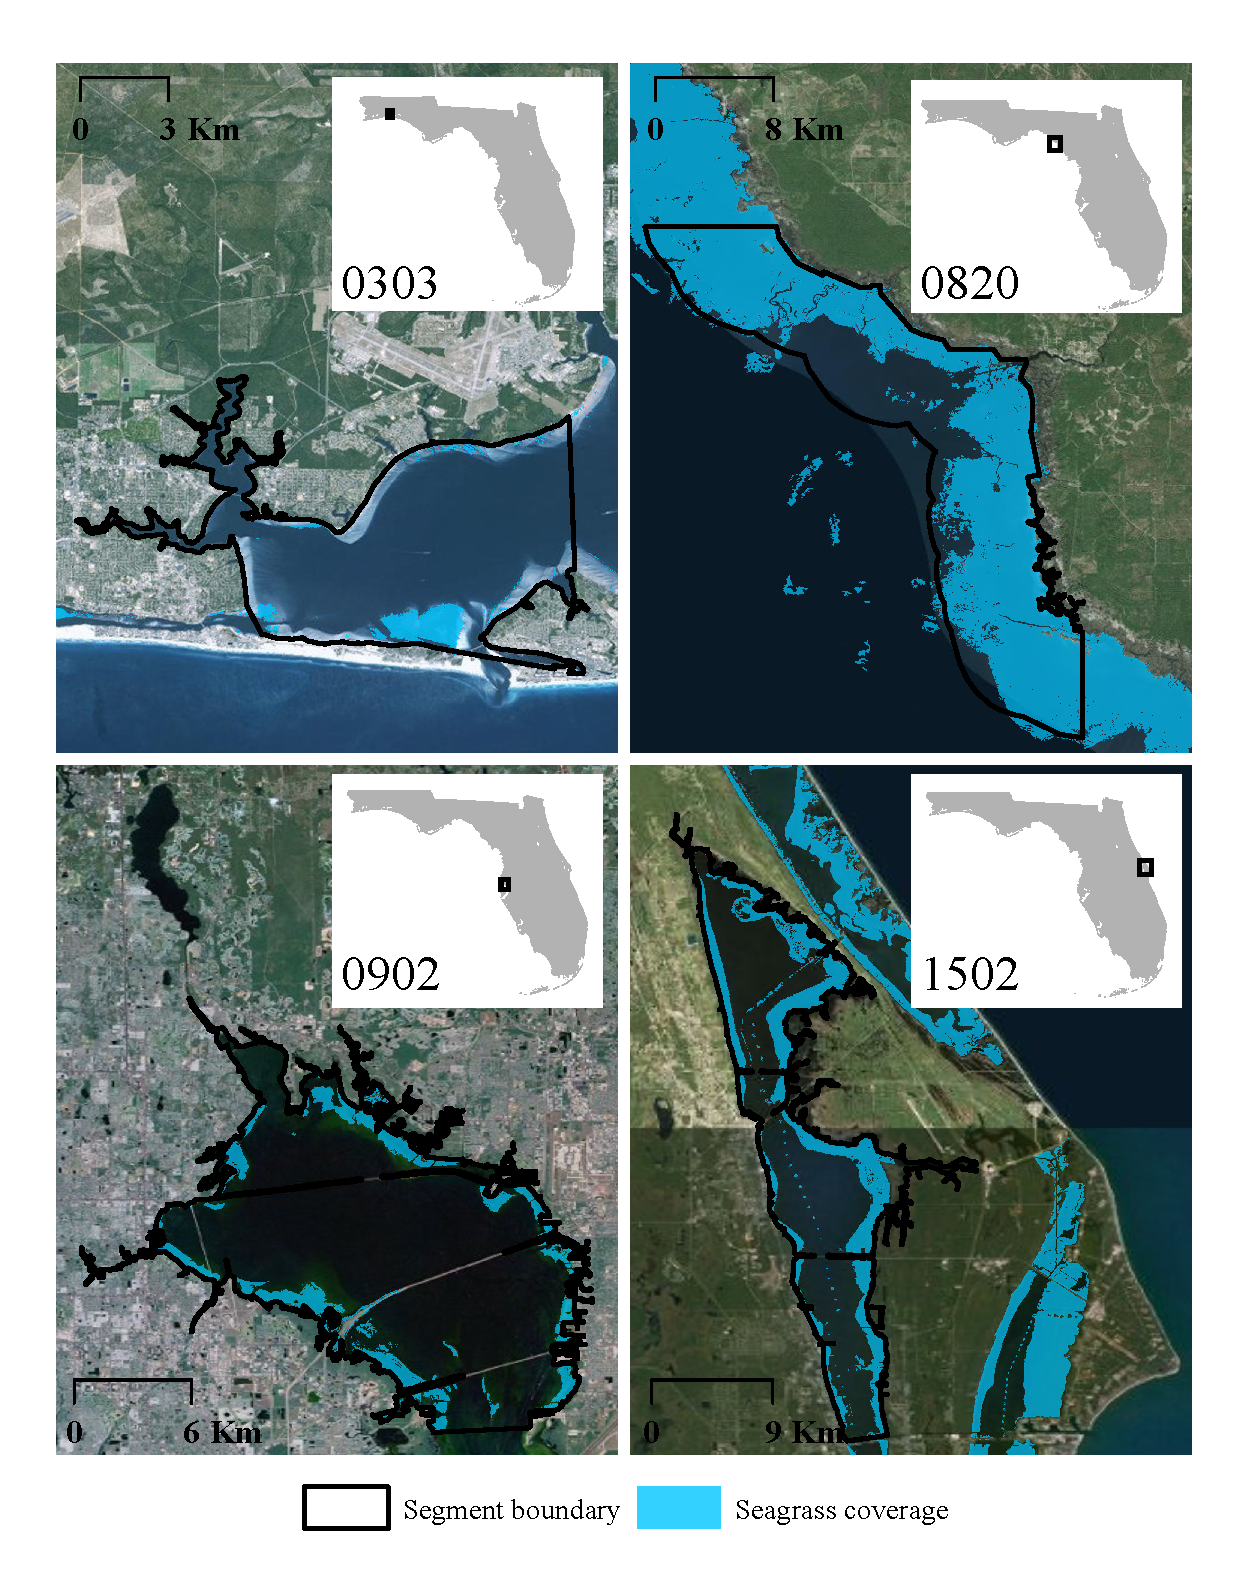
\includegraphics[width = \textwidth]{figs/seg_all.pdf}}
\caption{Locations and seagrass coverage of estuary segments used to evaluate \acl{doc} estimates.  Seagrass coverage layers are from 2007 (Choctowatchee Bay, 0303), 2006 (Big Bend, 0820), 2010 (Old Tampa Bay, 0902), and 2009 (Indian River Lagoon, 1502).}
\label{fig:seg_all}
\end{figure}

% example of depth of col ests for wbid - big bend 820
\begin{figure}
\centerline{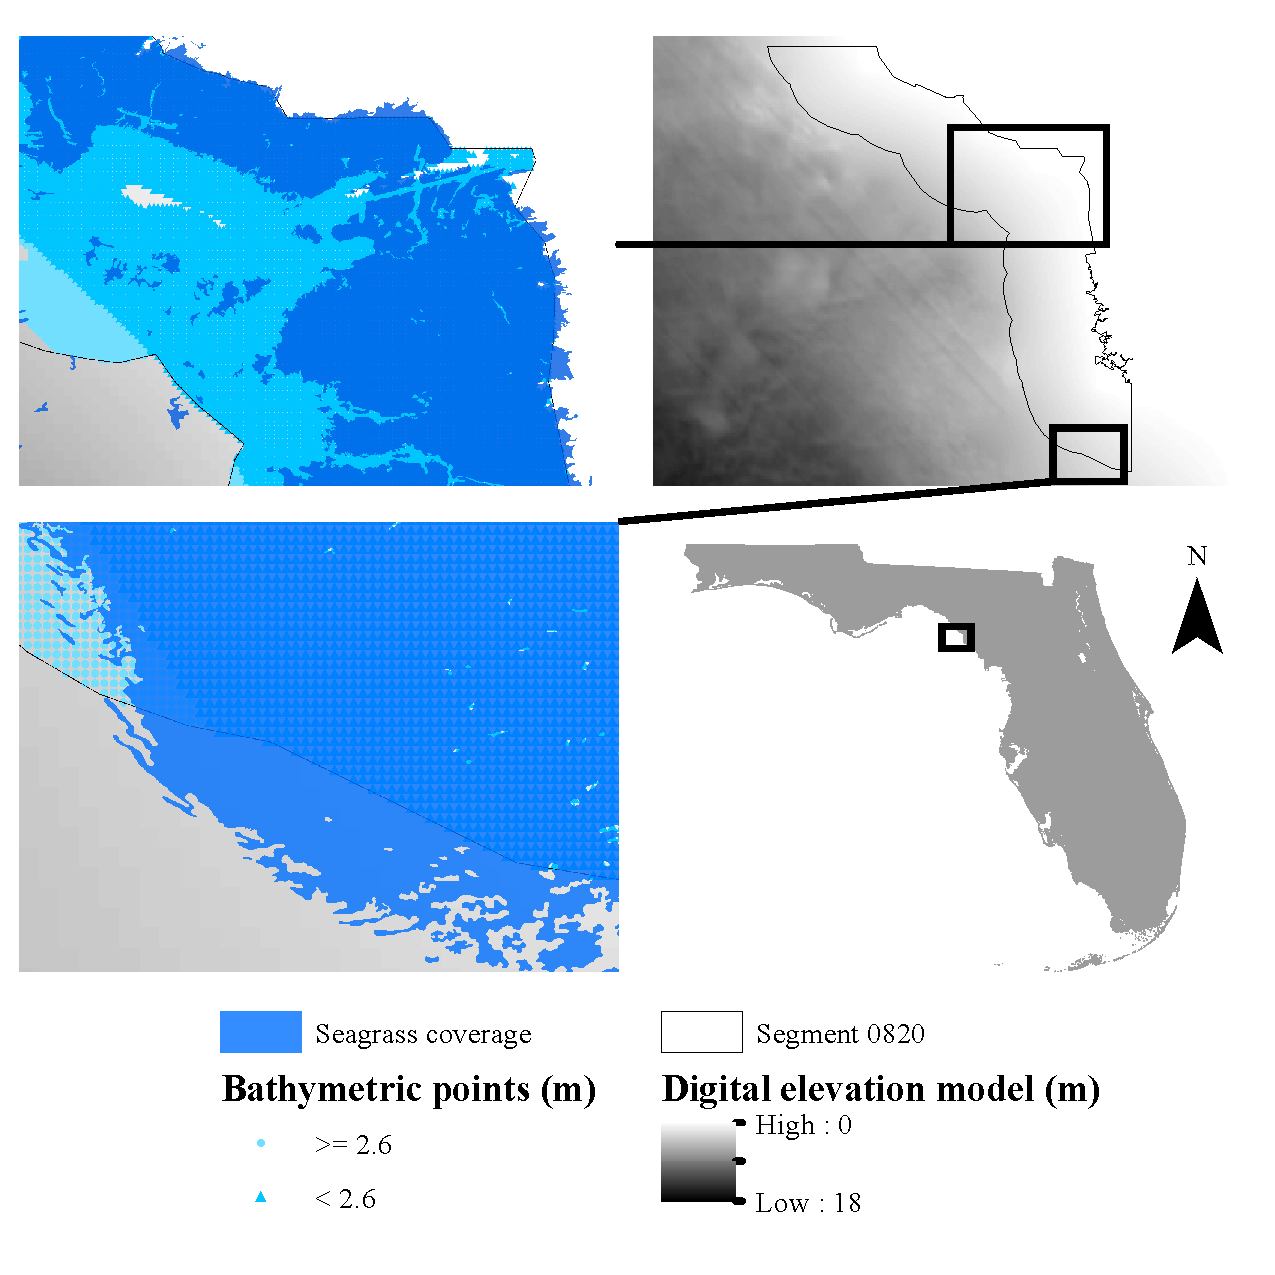
\includegraphics[width = \textwidth]{figs/wbid_doc.pdf}}
\caption{Example of over- and under-estimates for seagrass depth of colonization for segment 820 in the Big Bend region, Florida.  Layers include a seagrass coverage layer, bathymetric depth points, bathymetric digital elevation model, and spatial extents for the segment and Florida.  The top-left figure indicates over-estimation and the bottom-left indicates under-estimation.  Bathymetric points are color-coded by the median depth of colonization estimate for seagrass using data from the whole segment (2.6 m).}
\label{fig:wbid_doc}
\end{figure}

% example of buffer points for depth of col


% example of buffer points for depth of col
\begin{figure}
\centering
\subfloat[][Seagrass depth points for the segment]{
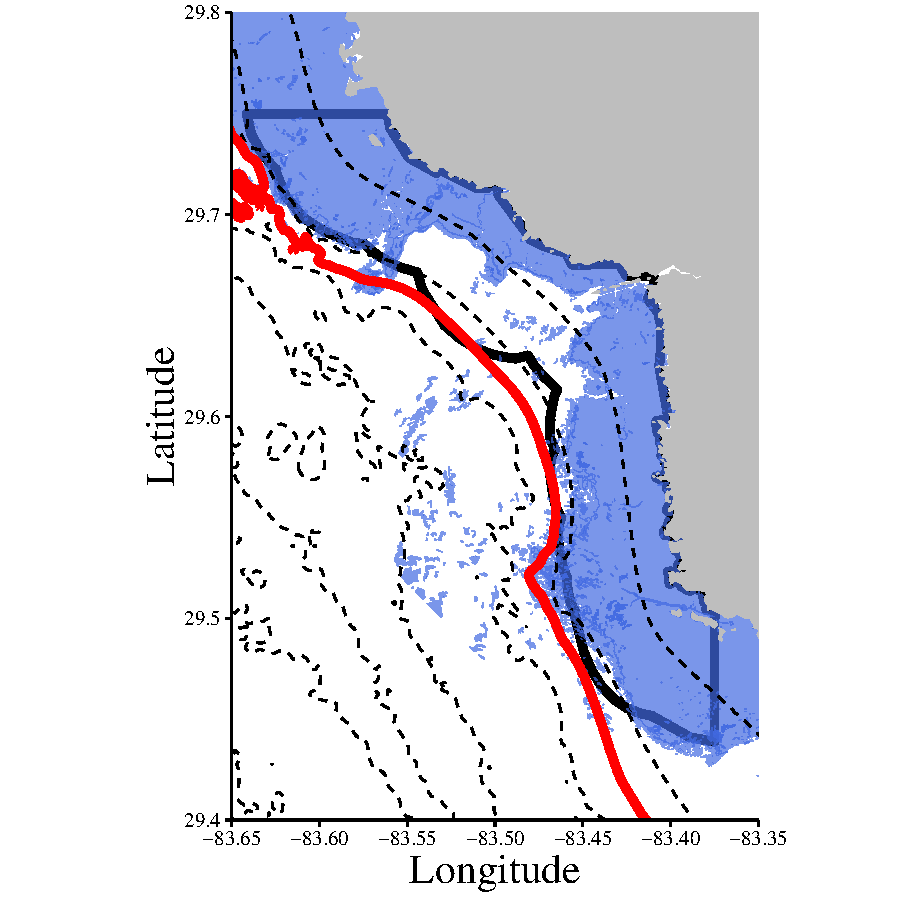
\includegraphics[width=0.5\textwidth, page = 1]{figs/buff_ex.pdf}
\label{fig:buff_ex1}
}
\subfloat[][Grid of locations and sample areas for estimates]{
\includegraphics[width=0.5\textwidth, page = 2]{figs/buff_ex.pdf}
\label{fig:buff_ex2}
}

\subfloat[][Sampled observations for a test point]{
\includegraphics[width=0.5\textwidth, page = 3]{figs/buff_ex.pdf}
\label{fig:buff_ex3}
}
\subfloat{
\includegraphics[width = 0.5\textwidth, page = 4]{figs/buff_ex.pdf}
}
\caption{Examples of data and grid locations for estimating seagrass depth of colonization for a region of the Big Bend, Florida.  \Cref{fig:buff_ex1} shows the seagrass depth points that are used for sampling, \cref{fig:buff_ex2} shows a grid of locations and sampling radii for estimating seagrass \ac{doc}, and \cref{fig:buff_ex3} shows an example of sampled seagrass depth points for a location.  Estimates in \cref{fig:est_ex} were obtained from the sampled location in \cref{fig:buff_ex3}.}
\label{fig:buff_ex}
\end{figure}

% example of estimating seagrass depth of colonization


% example of depth of col ests for wbid - big bend 820
\begin{figure}
\centering
\subfloat[][Proportion of points with seagrass by depth]{
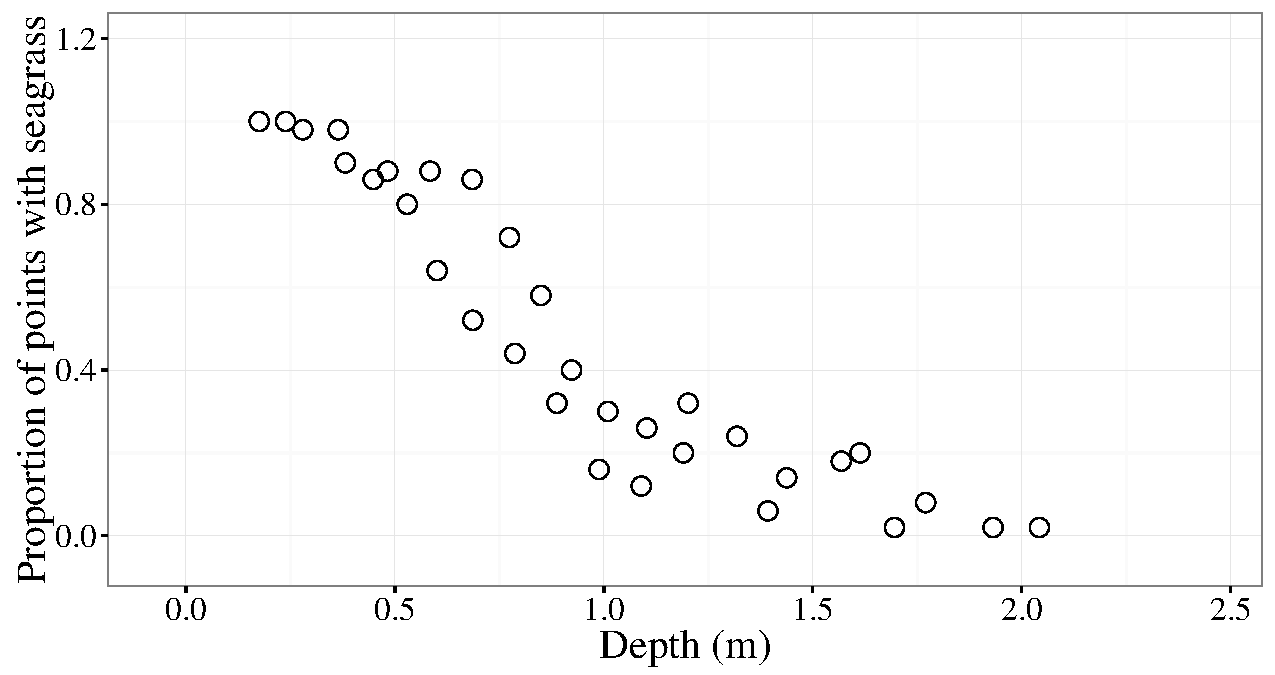
\includegraphics[page=1,width=0.5\textwidth]{figs/est_ex.pdf}
\label{fig:est_ex1}
}

\subfloat[][Logistic growth curve fit through points]{
\includegraphics[page=2,width=0.5\textwidth]{figs/est_ex.pdf}
\label{fig:est_ex2}
}

\subfloat[][Depth estimates]{
\includegraphics[page=3,width=0.5\textwidth]{figs/est_ex.pdf}
\label{fig:est_ex3}
}
\caption{Methods for estimating seagrass depth of colonization using sampled seagrass depth points around a single location. \Cref{fig:est_ex1} is the proportion of points with seagrass by depth using depth points within the buffer of the test point in \cref{fig:buff_ex}.  \Cref{fig:est_ex2} adds a decreasing logistic growth curve fit through the points.  \Cref{fig:est_ex3} shows three depth estimates based on a linear curve fit through the inflection point of logistic growth curve.}
\label{fig:est_ex}
\end{figure}

% grid examples for each segment

\begin{figure}
\centering
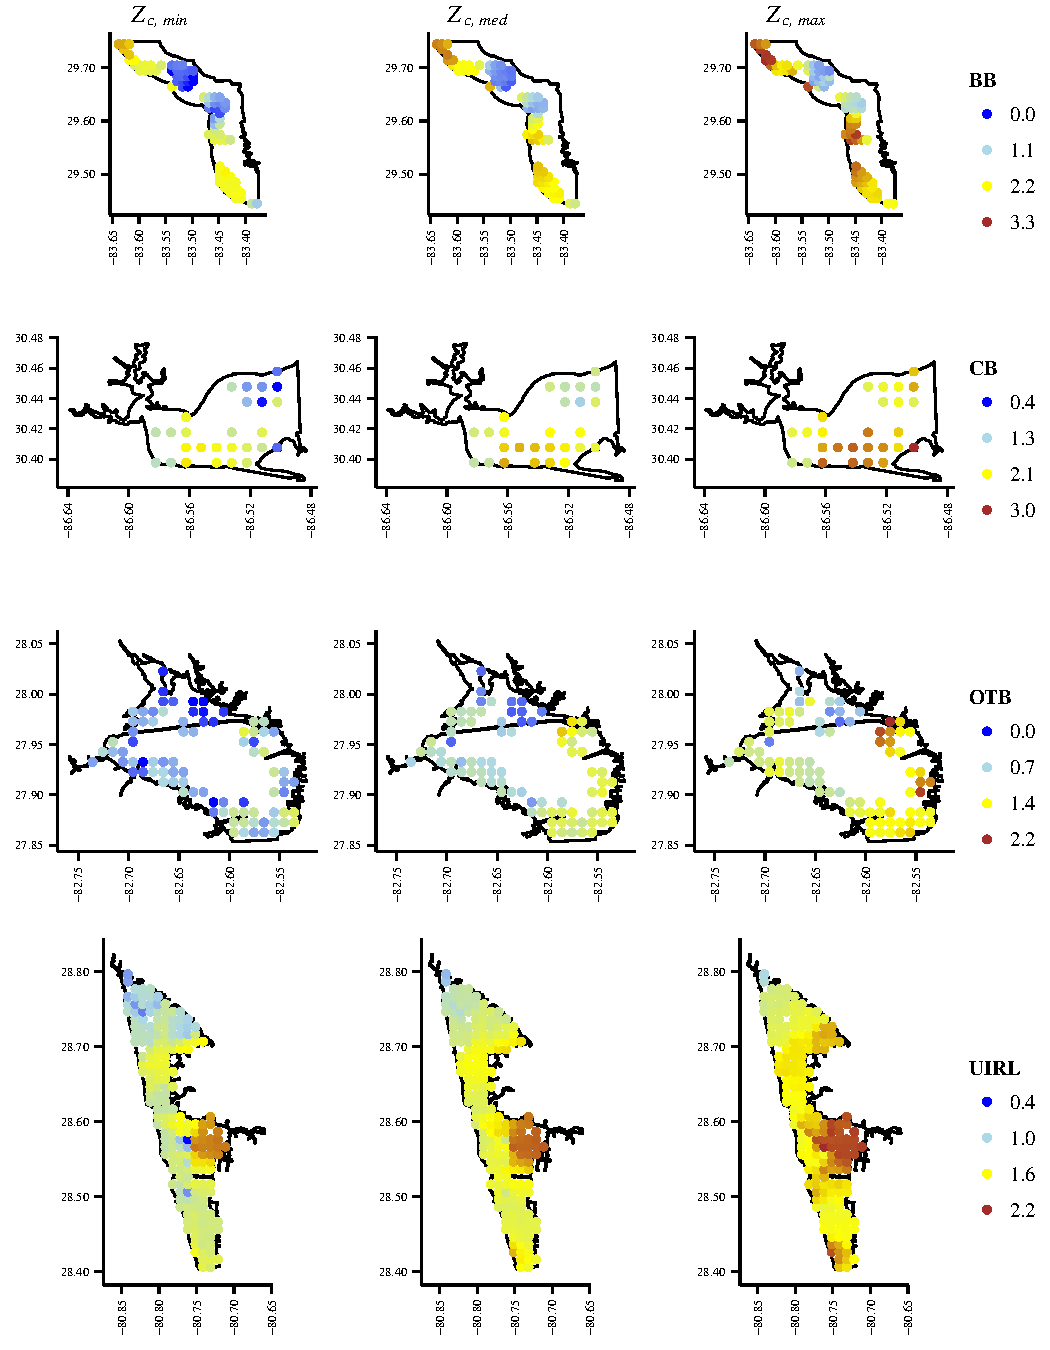
\includegraphics[width = 0.95\textwidth]{figs/all_ests.pdf}
\caption{Spatially-referenced estimates of seagrass depth limits (m) for four coastal segments of Florida.  Estimates include minimum ($Z_{min}$), median ($Z_{med}$), and maximum depth of colonization ($Z_{max}$).  Estimates are assigned to grid locations for each segment, where grid spacing was fixed at 0.02 decimal degrees.  Radii for sampling seagrass bathymetric data around each grid location were fixed at 0.06 decimal degrees.}
\label{fig:all_ests}
\end{figure}

% range of confidence intervals for estimates

\begin{figure}
\centering
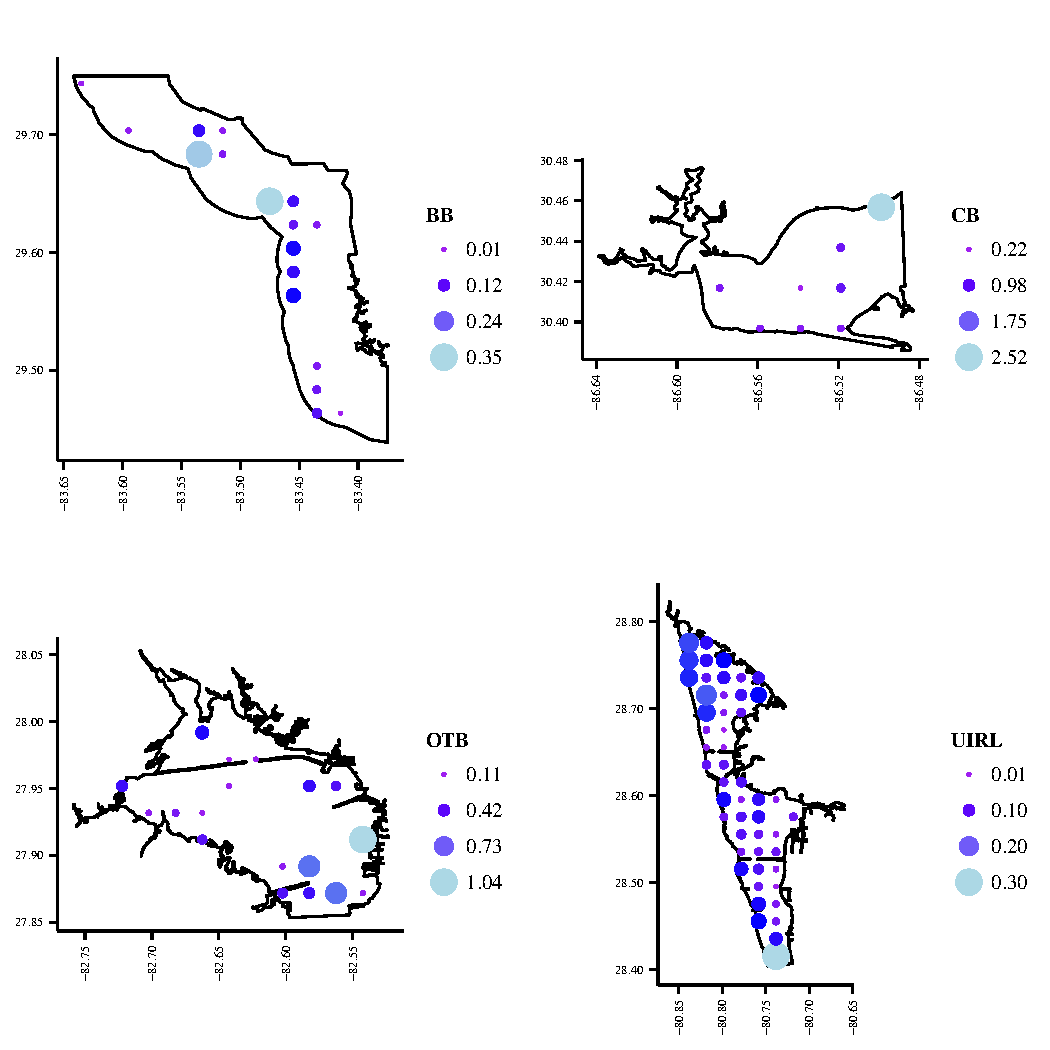
\includegraphics[width = 0.95\textwidth]{figs/all_sens.pdf}
\caption{Size of confidence intervals (m) for \acl{doc} estimates in \cref{fig:all_ests}.  Points are colored and sized based on the difference between the upper and lower bounds of a 95\% confidence interval for all three \ac{doc} estimates ($Z_{min}$, $Z_{med}$, $Z_{max}$). Bounds were obtained using Monte Carlo simulations to estimate uncertainty associated with the inflection point of the estimated logistic curve (\cref{fig:est_ex}) for each sample.}
\label{fig:all_sens}
\end{figure}

% estimated light requirements for Tampa Bay

\begin{figure}
\centering
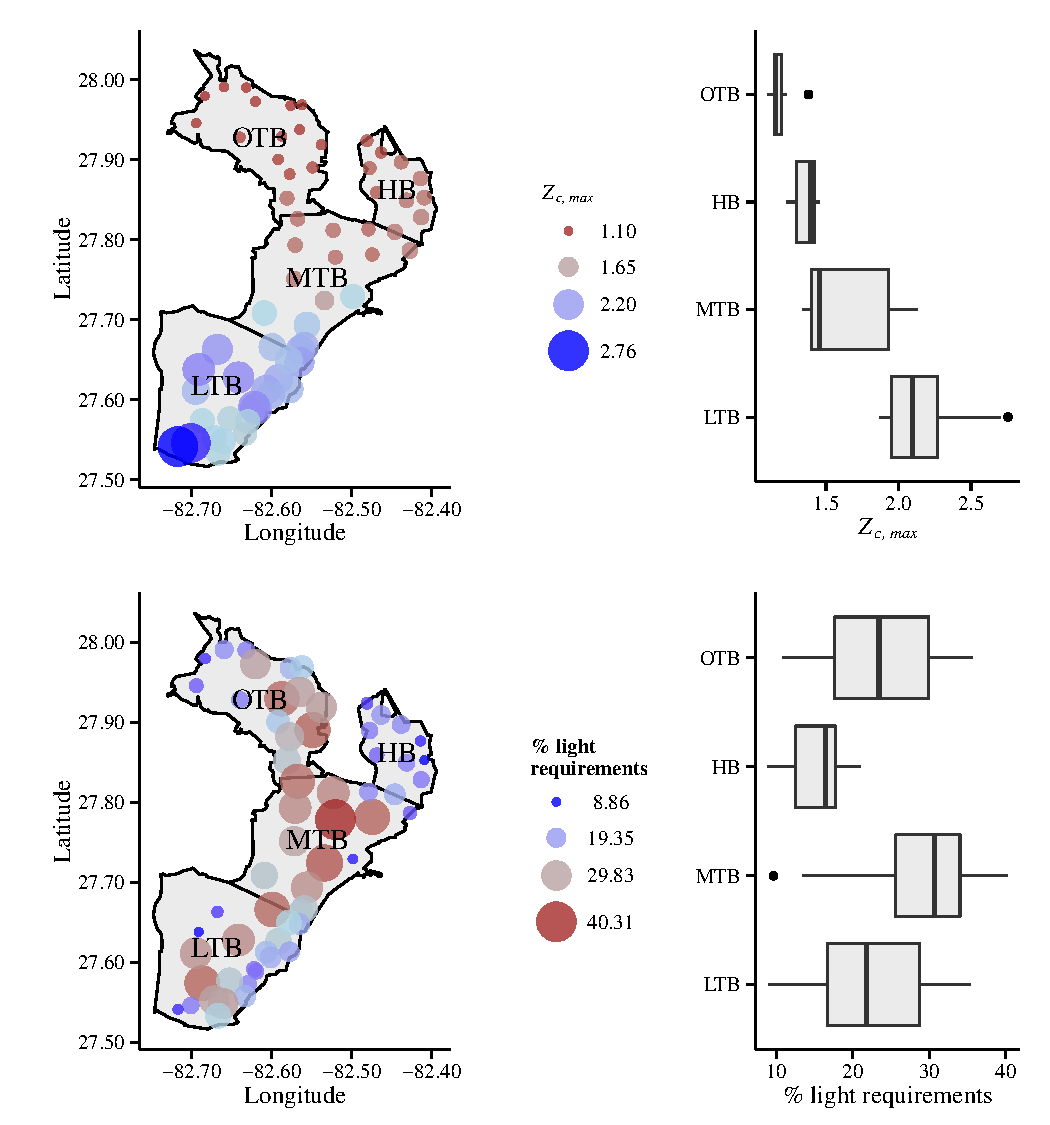
\includegraphics[width = 0.95\textwidth]{figs/light_tb.pdf}
\caption{Estimated light requirements of seagrass for multiple locations in Tampa Bay, Florida.  Map locations are georeferenced observations of water clarity from secchi measurements in the Florida \acl{IWR} database, update 40.  Data are also summarized by bay segment as boxplots where the dimensions are the 25\textsuperscript{th} percentile, median, and 75\textsuperscript{th} percentile.  Whiskers extend beyond the boxes as 1.5 multiplied by the interquartile range.  Light requirements are based on daily average secchi values for each location using all observations for Tampa Bay, estimated maximum depth of colonization using a radius of 0.7 decimal degrees for each secchi location to sample seagrass depth points for 2010 coverage data, and empirical relationships described by \cref{eqn:lambeer}. HB: Hillsborough Bay, LTB: Lower Tampa Bay, MTB: Middle Tampa Bay, OTB: Old Tampa Bay.}
\label{fig:light_tb}
\end{figure}

% estimated light requirements for Indian River Lagoon

\begin{figure}
\centering
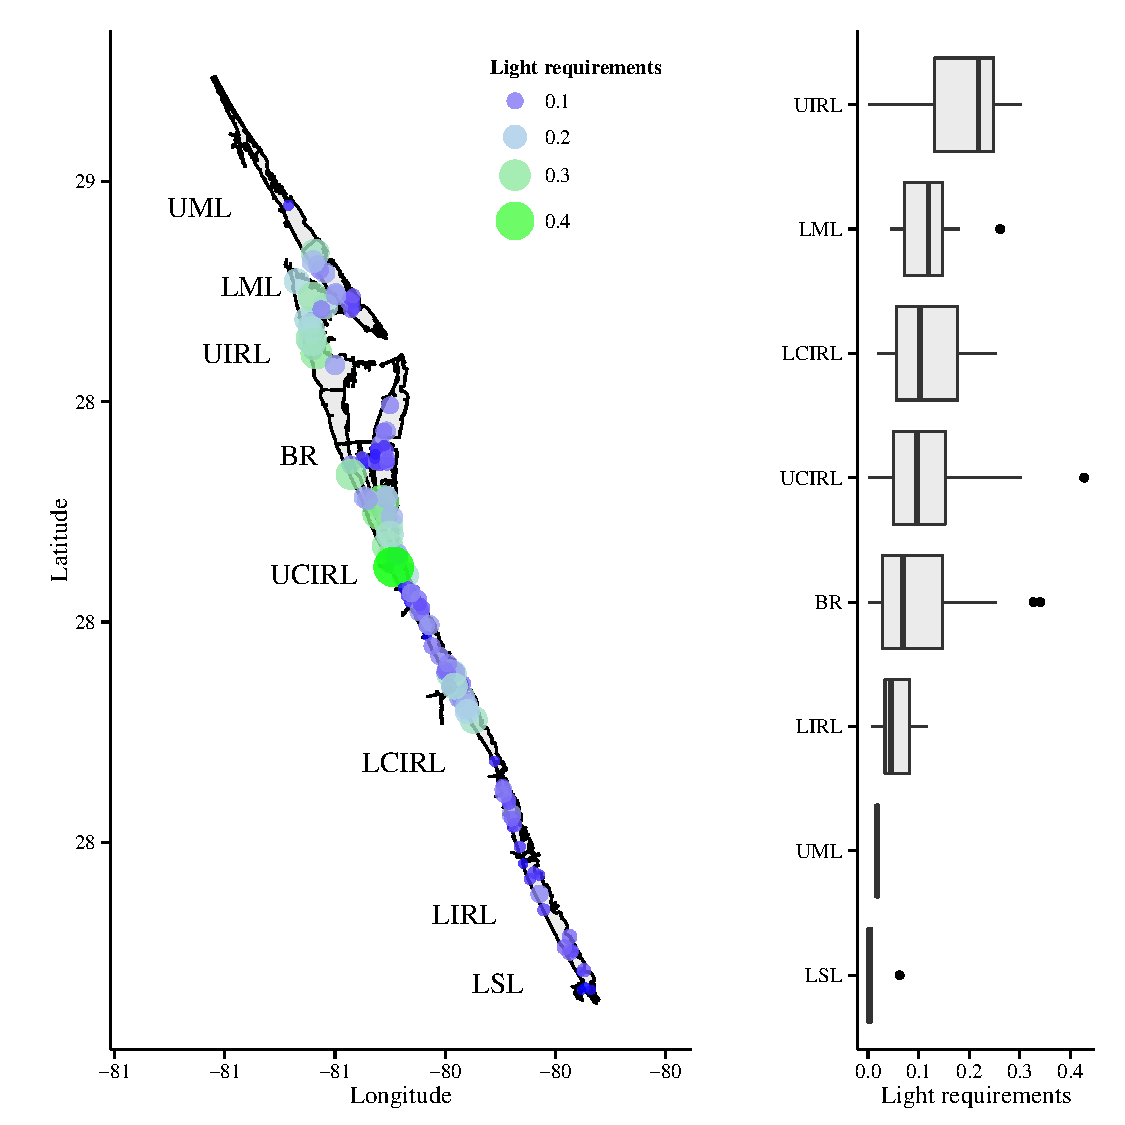
\includegraphics[width = \textwidth]{figs/light_irl.pdf}
\caption{Estimated light requirements of seagrass for multiple locations in Indian River Lagoon, Florida.  Map locations are georeferenced observations of water clarity from secchi measurements in the Florida \acl{IWR} database, update 40.  Data are also summarized by bay segment as boxplots as in \cref{fig:light_tb}. Light requirements are based on daily average secchi values for each location using all observations for Tampa Bay, estimated maximum depth of colonization using a radius of 0.02 decimal degrees for each secchi location to sample seagrass depth points for 2009 coverage data, and empirical relationships described by \cref{eqn:lambeer}. BR: Banana R., LCIRL: Lower Central Indian R. Lagoon, LIRL: Lower Indian R. Lagoon, LML: Lower Mosquito Lagoon, LSL: Lower St. Lucie, UCIRL: Upper Central Indian R. Lagoon, UIRL: Upper Indian R. Lagoon, UML: Upper Mosquito Lagoon.}
\label{fig:light_irl}
\end{figure}


\end{document}
